\documentclass{article}
\usepackage{ctex}
\usepackage{graphicx}
\usepackage{ctex}
\usepackage{amsmath}
\usepackage{amsfonts}
\usepackage{amssymb}
\usepackage{enumerate}
\usepackage{color}
\usepackage{setspace}
\usepackage{pythonhighlight}
\usepackage{bm}

\usepackage
[a4paper,
text={146.4true mm,239.2 true mm},
top= 26.2true mm,
left=31.8 true mm,
head=6true mm,
headsep=6.5true mm,
foot=16.5true mm]
{geometry} % 设置文本的边距
\input{../setup/format}

\begin{document}
    \title{Homework 7 of Stochastic Processes}
    \author{姓名:林奇峰\qquad 学号:19110977}
    \maketitle

    \section{Exercise 4.22}
    \begin{figure}[h]
        \centering
        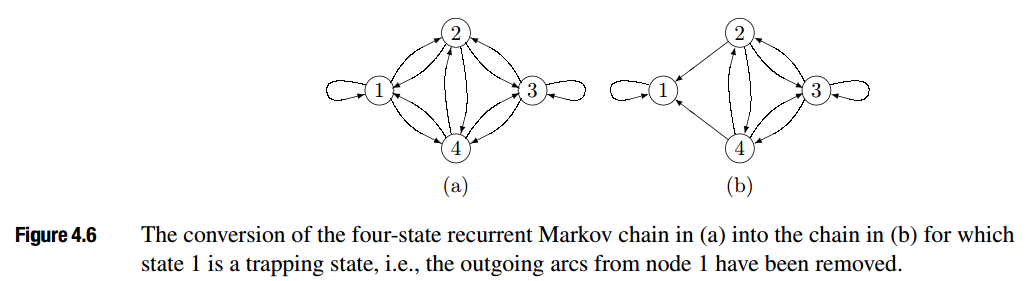
\includegraphics[width=5.9in]{figure_4_6.png}
    \end{figure}
    Section 4.5.1 showed how to find the expected first-passage times to a fixed state, say 1, from all other states. It is often desirable to include the expected first recurrence time from state 1 to return to state 1. This can be done by splitting state 1 into two states, first an initial state with no transitions coming to it but the original transitions going out, and, second, a final trapping state with the original transitions coming in.
    \begin{enumerate}[(a)]
        \item For the chain on the left side of Figure 4.6, draw the graph for the modified chain with five states where state 1 has been split into two states.
        \item Suppose one has found the expected first-passage times $\nu_j$ for states $j=2,\dots,4$ (or in general from 2 to M). Find an expression for $\nu_1$, the expected first recurrence time for state 1 in terms of $\nu_2,\nu_3,\dots,\nu_\text{M}$ and $P_{12},\dots,P_{1\text{M}}$.
    \end{enumerate}

    \textbf{Solutions:}

    \begin{enumerate}[(a)]
        \item 
        Picture:
        \begin{figure}[h]
            \centering
            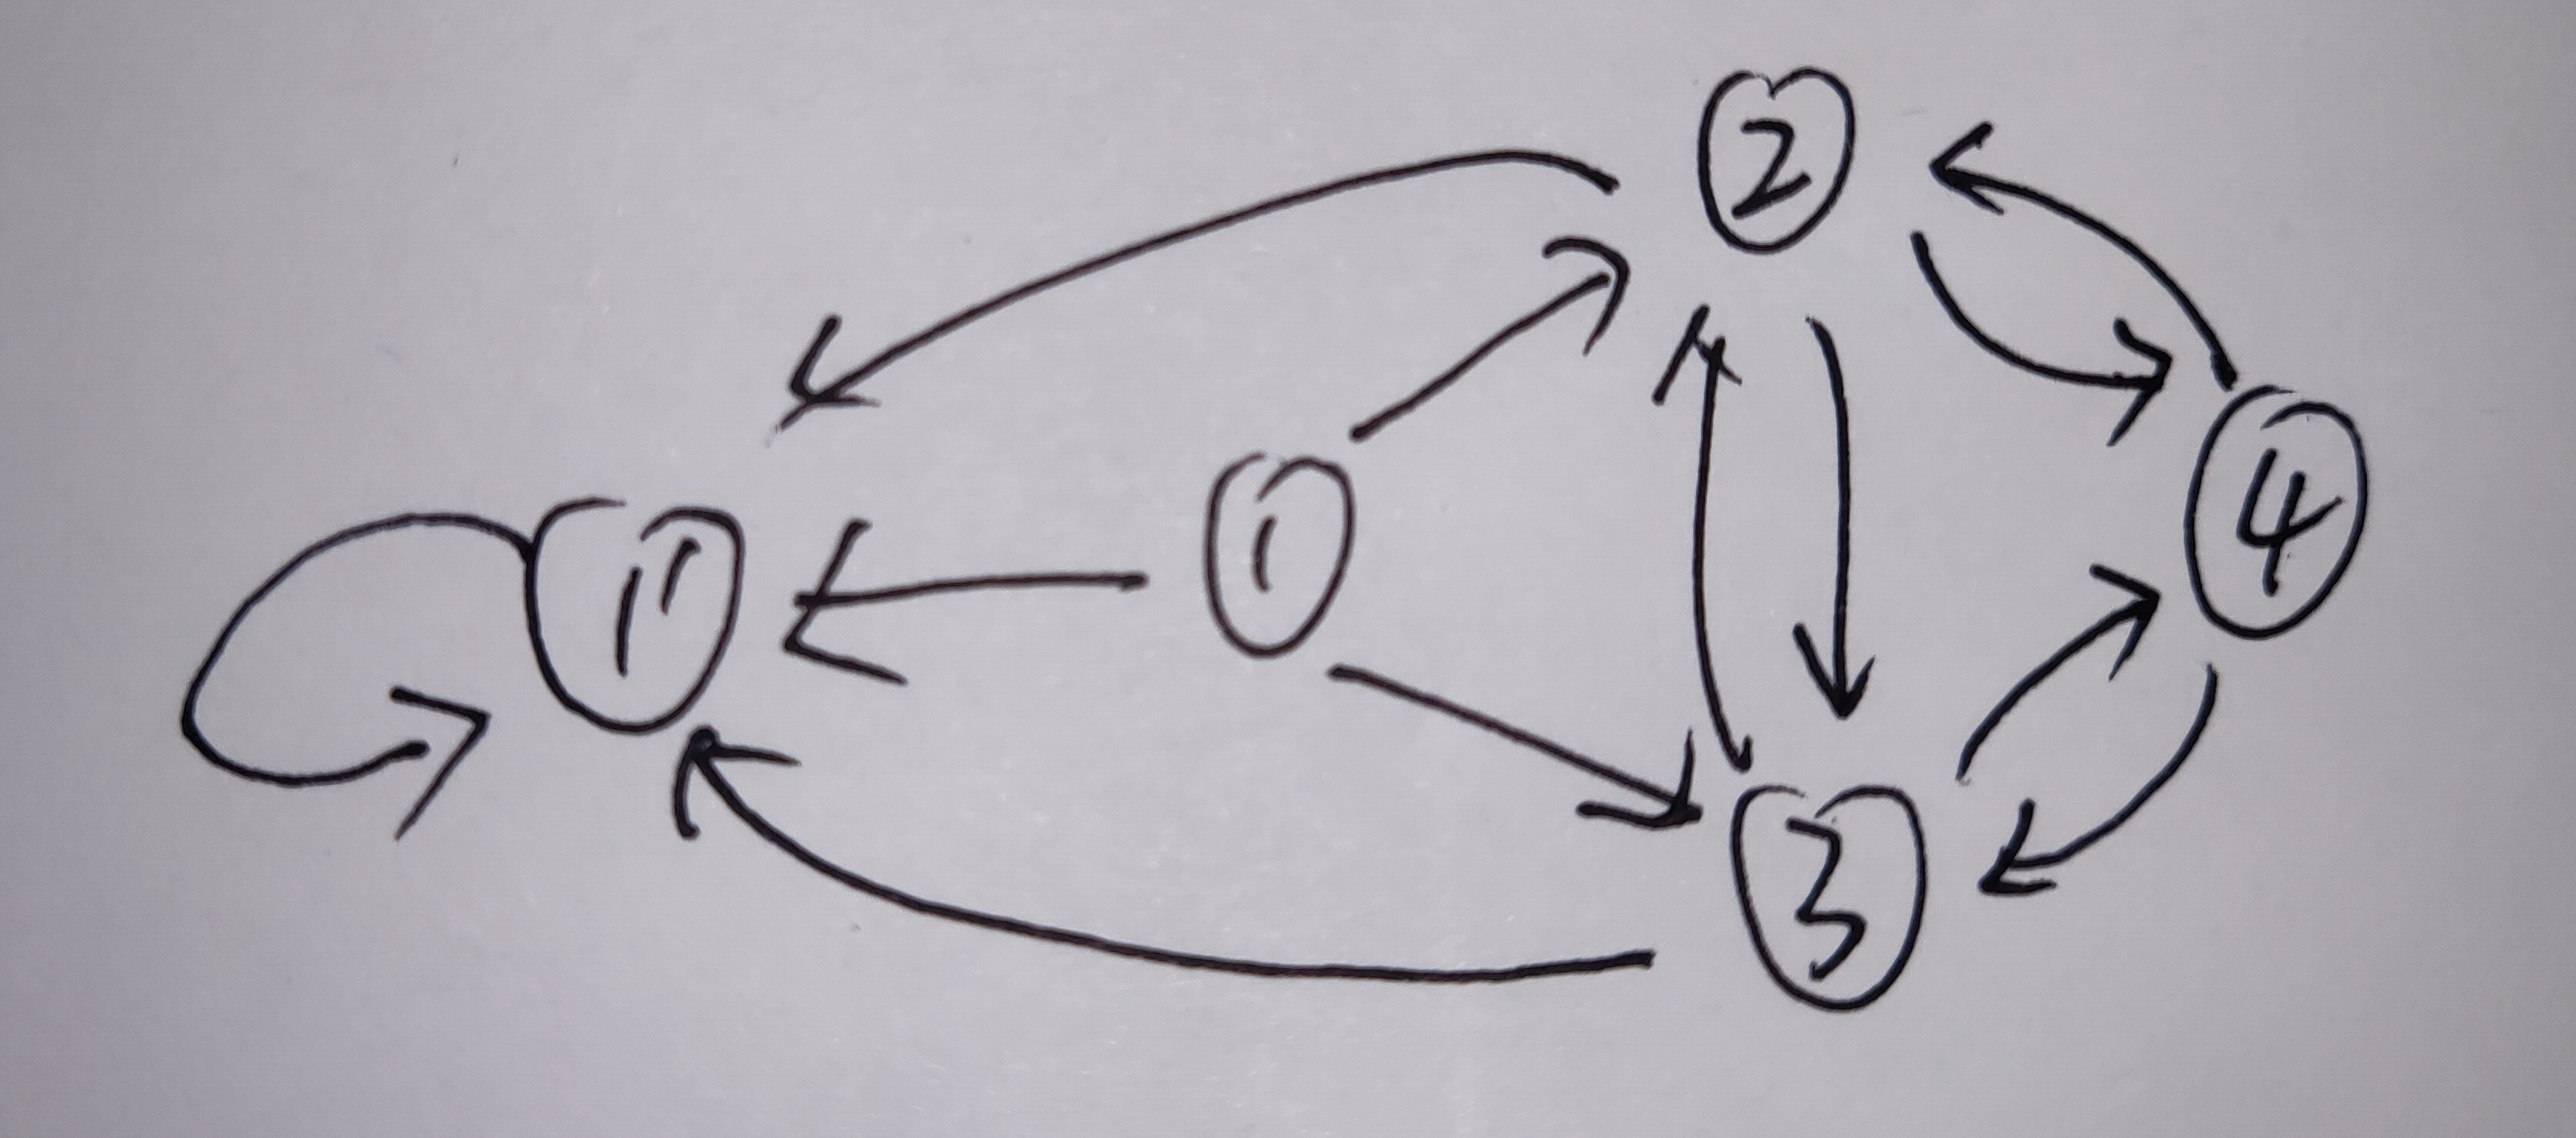
\includegraphics[width=3.0in]{1.jpg}
        \end{figure}
        \item   \begin{equation*}
                    \nu_1=1+\sum_{j=2}^4P_{1j}\nu_j
                \end{equation*}
    \end{enumerate}

    \section{Exercise 4.28}
    Consider finding the expected time until a given string appears in a IID binary sequence with $\text{Pr}\{X_n=1\}=p_1,\text{Pr}\{X_n=0\}=p_0=1-p_1$.
    \begin{enumerate}[(a)]
        \item Following the procedure in Example 4.5.1, draw the three-state Markov chain for the string (0,1). Find the expected number of trials unitl the first occurence of the string.
        \item For (b) and (c), let $(a_1,a_2,a_3,\dots,a_k)=(0,1,1,\dots,1)$, i.e., zero followed by $k-1$ ones. Draw the corresponding Markov chain for $k=4$.
        \item Let $\nu_i,1\leq i\leq k$ be the expected first-passage time from state $i$ to state $k$. Note that $\nu_k=0$. For each $i, 1\leq i\leq k$, show that $\nu_i=\alpha_i+\nu_{{i+1}}$ and $\nu_0=\beta_i+\nu_{i+1}$, where $\alpha_i$ and $\beta_i$ are each expressed as a product of powers of $p_0$ and $p_1$. Hint: Use induction on $i$ taking $i=1$ as the base. For the inductive step, first find $\beta_{i+1}$ as a function of $\beta_i$ starting with $i=1$ and using the equation $\nu_0=1/p_0+\nu_1$.
        \item Let $\bm{a}=(0,1,0)$. Draw the corresponding Markov chain for this string. Evaluate $\nu_0$, the expected time for (0,1,0) to occur. 
    \end{enumerate}

    \textbf{Solutions:}
    \begin{enumerate}[(a)]
        \item 
        Picture:
        \begin{figure}[h]
            \centering
            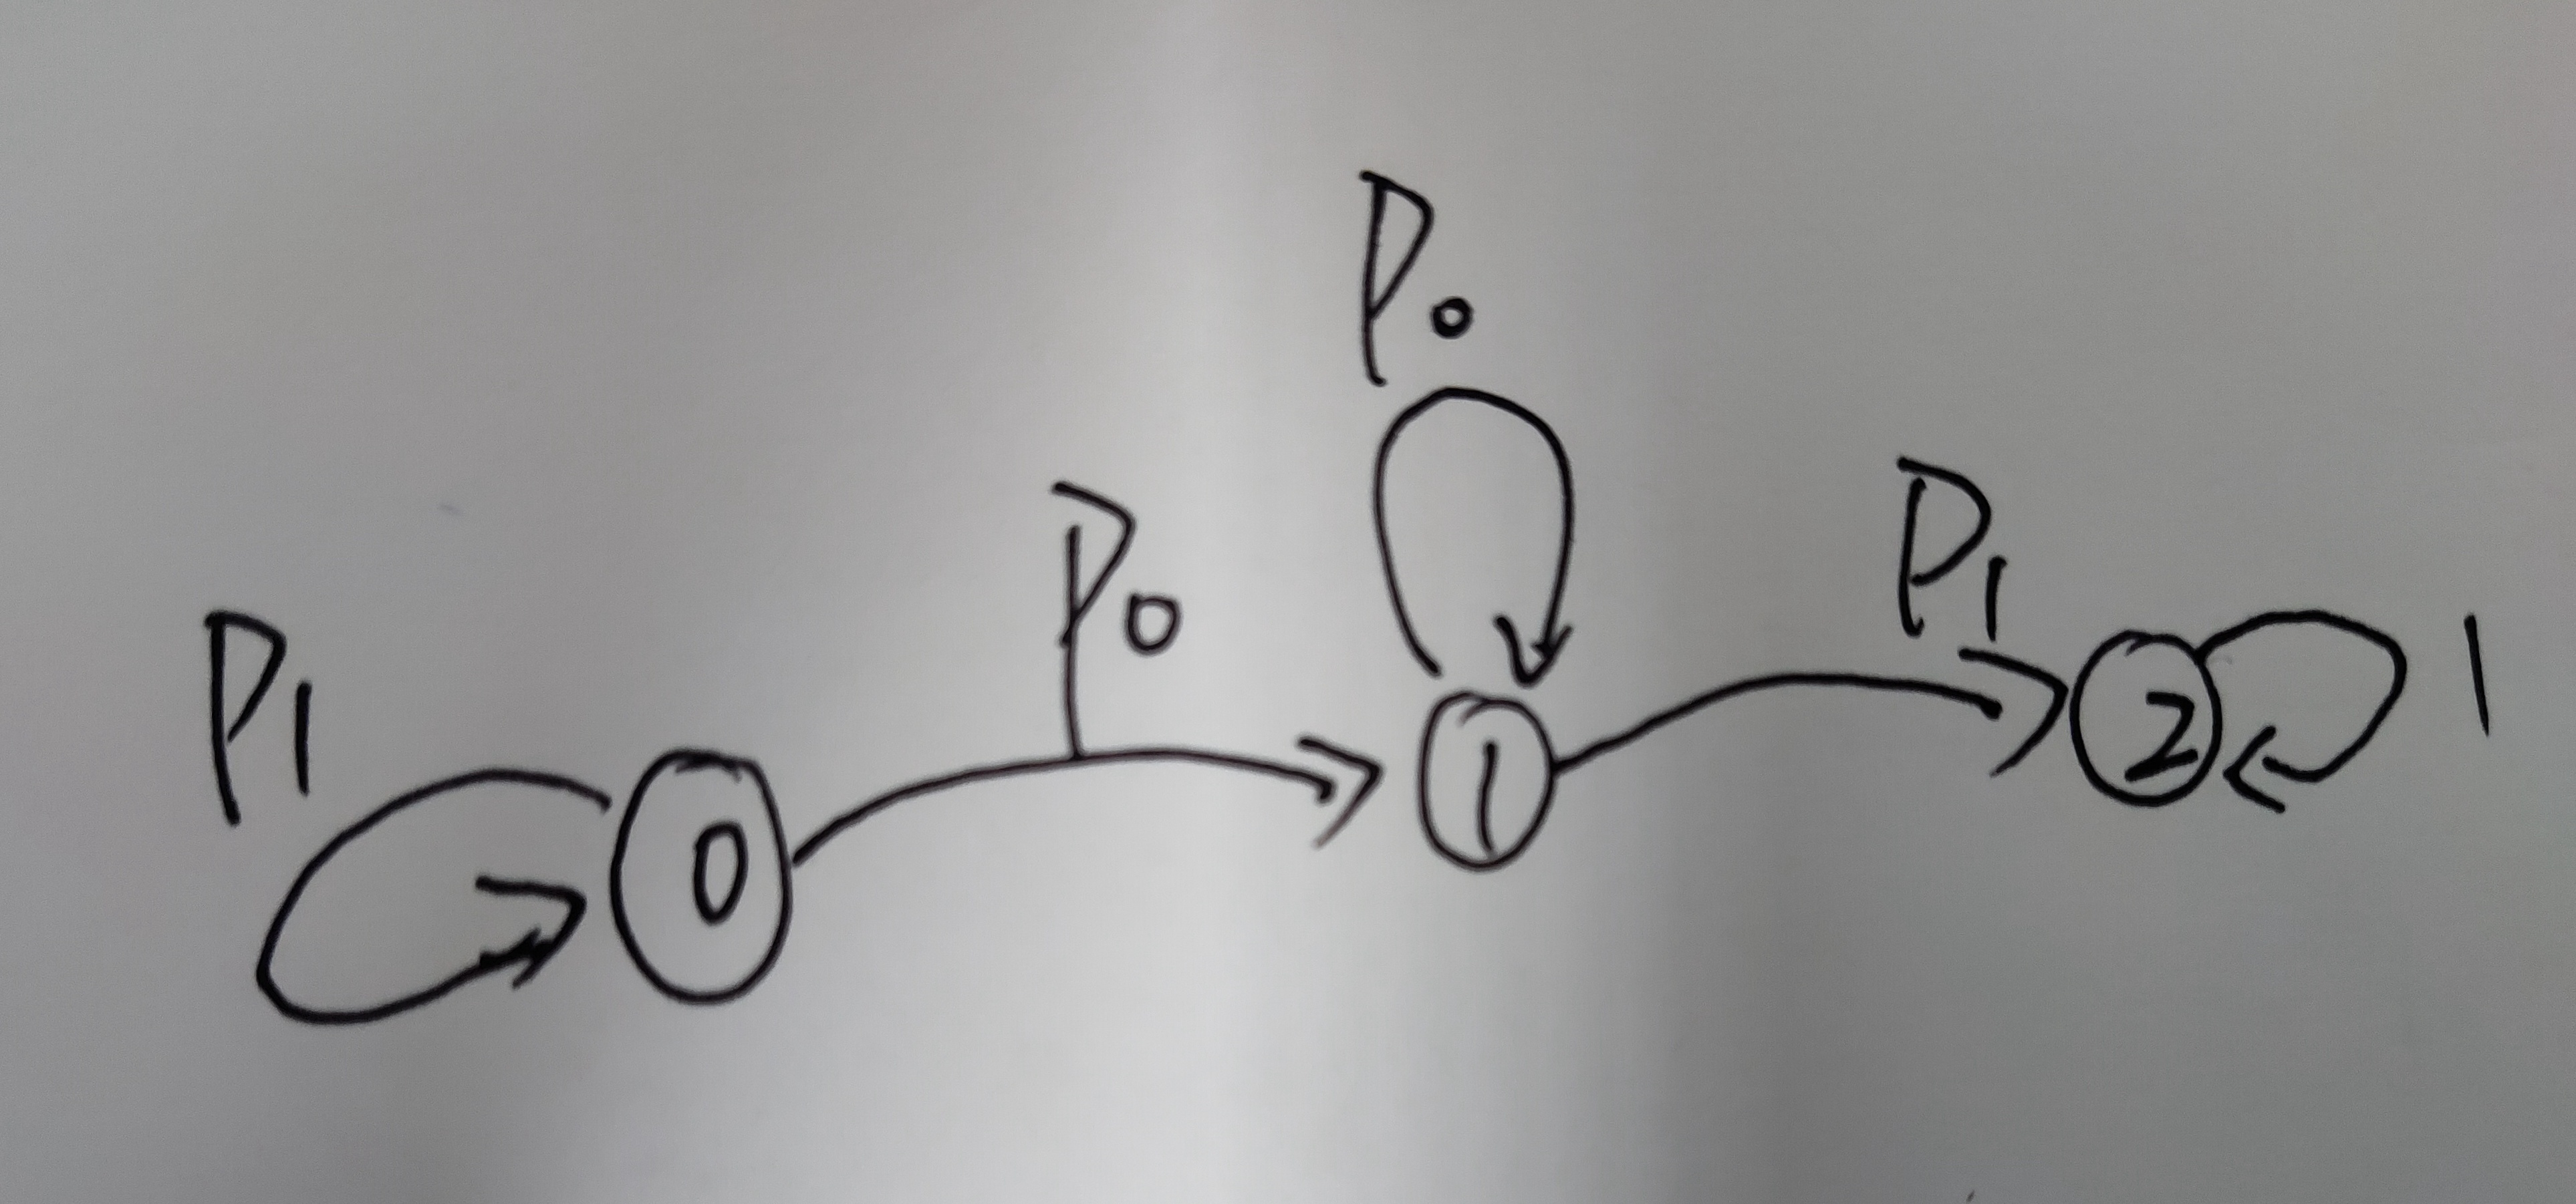
\includegraphics[width=3.0in]{2.jpg}
        \end{figure}

        We can obtain the following equations, 
        \begin{equation*}
            \begin{aligned}
                \nu_0 &= 1+p_1\nu_0+p_0\nu_1\\
                \nu_1 &= 1+p_0\nu_1+p_1\nu_2\\
                \nu_2 &= 0
            \end{aligned}
        \end{equation*}

        Solve the equal equations,
        \begin{equation*}
            \begin{aligned}
                \nu_0 - \nu_1 &= \frac{1}{p_0}\\
                \nu_1 - \nu_2 &= \frac{1}{p_1}\\
                \nu_2 &= 0
            \end{aligned}
        \end{equation*}

        Finally,
        \begin{equation*}
            \begin{aligned}
                \nu_0 &= \frac{1}{p_0p_1}
            \end{aligned}
        \end{equation*}
        \item 
        Picture:
        \begin{figure}[h]
            \centering
            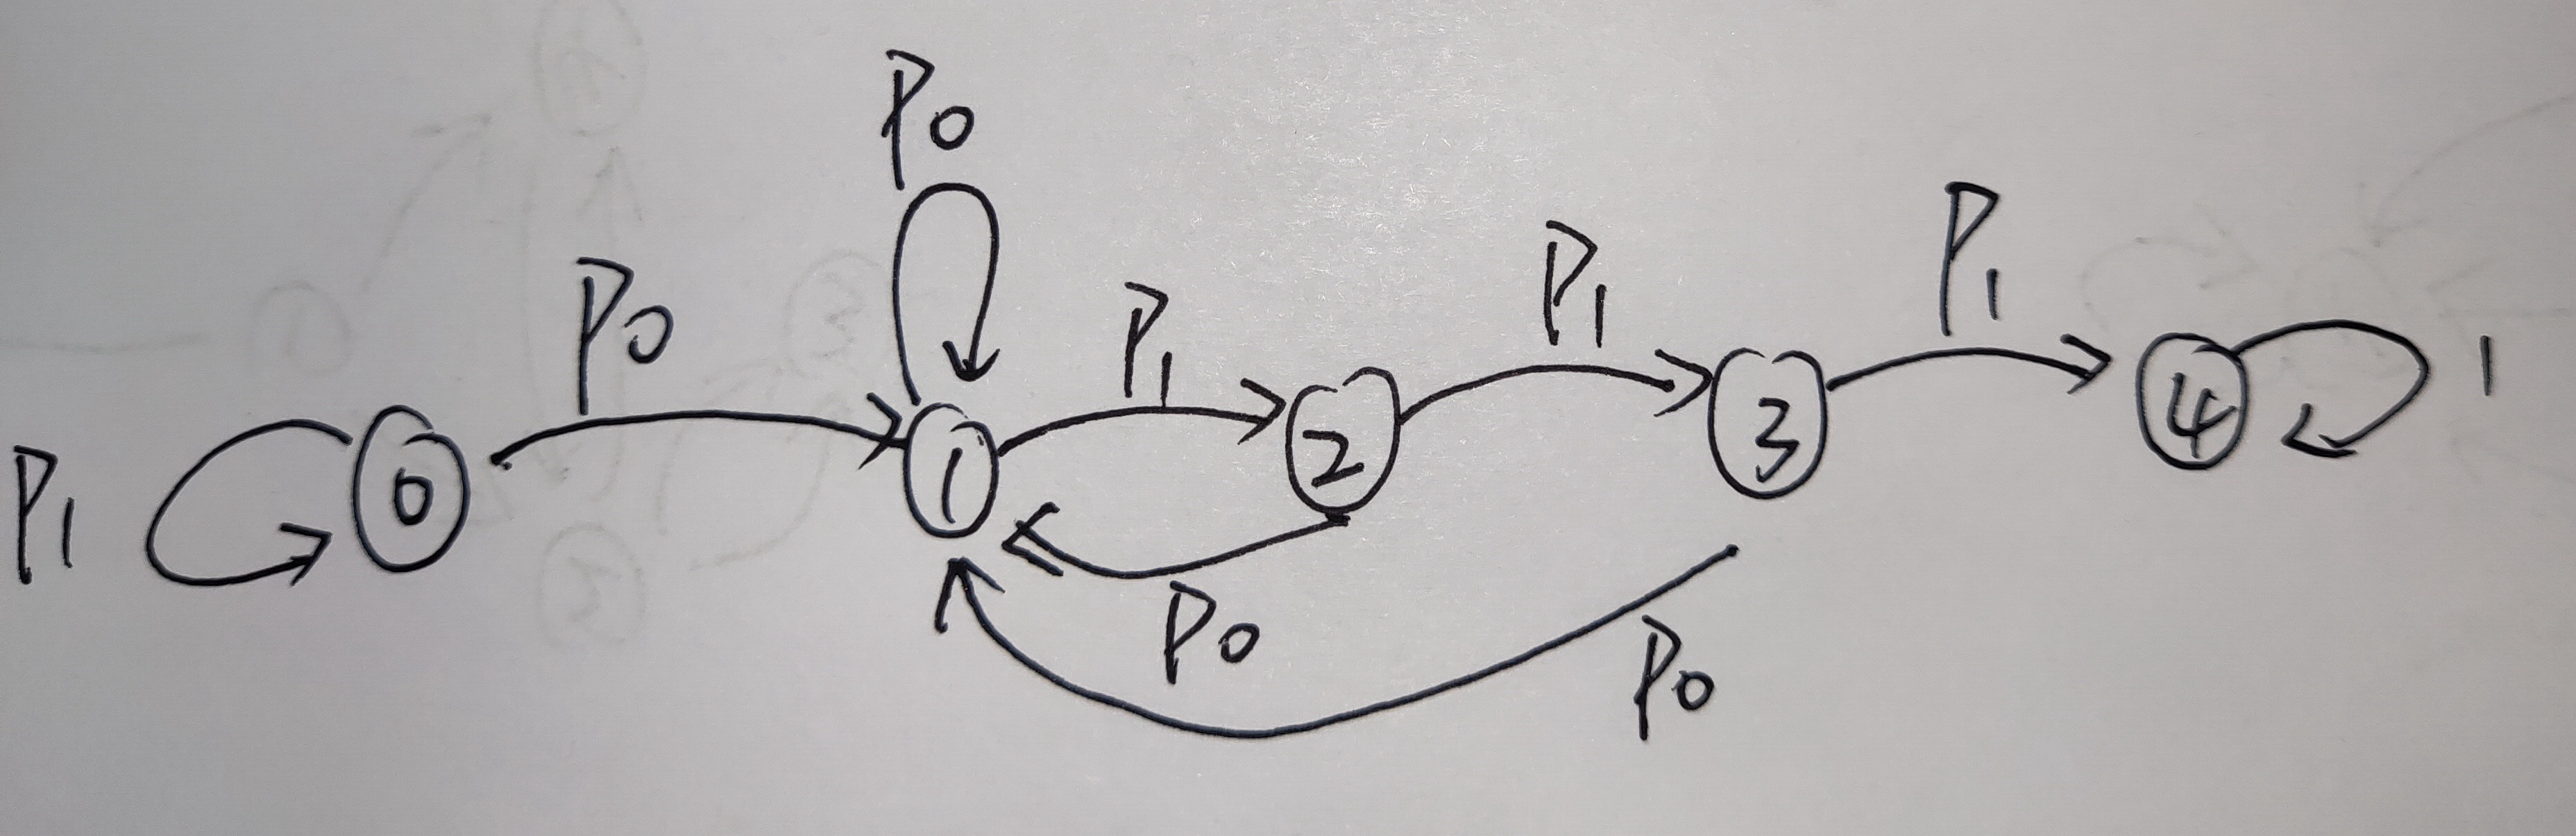
\includegraphics[width=4.0in]{3.jpg}
        \end{figure}
        \item From (a), we can know that
        \begin{equation*}
            \begin{aligned}
                \alpha_1&=\frac{1}{p_1}\\
                \beta_1&=\frac{1}{p_0p_1}
            \end{aligned}
        \end{equation*}

        Assume that $\nu_i=\alpha_i+\nu_{i+1}$ and $\nu_0=\beta_i+\nu_{i+1}$ hold for each $i,1\leq i\leq k$, then 
        \begin{equation*}
            \begin{aligned}
                \nu_{i+1}&=1+p_0\nu_1+p_1\nu_{i+2}\quad\text{which can be seen from (b)}\\
                &=p_0\nu_0+p_1\nu_{i+2}\\
                &=p_0(\beta_i+\nu_{i+1})+p_1\nu_{i+2}\\
                &=p_0\beta_i+p_0\nu_{i+1}+p_1\nu_{i+2}\\
                &\Downarrow\\
                \nu_{i+1}&=\frac{p_0\beta_i}{p_1}+\nu_{i+2}
            \end{aligned}
        \end{equation*}

        Therefore
        \begin{equation*}
            \alpha_{i+1}=\frac{p_0\beta_i}{p_1}
        \end{equation*}
        
        and
        \begin{equation*}
            \nu_0=\beta_i+\nu_{i+1}=\beta_i+\frac{p_0\beta_i}{p_1}+\nu_{i+2}=\frac{\beta_i}{p_1}+\nu_{i+2}
        \end{equation*}
        
        We can see that
        \begin{equation*}
            \beta_{i+1}=\frac{\beta_i}{p_1}
        \end{equation*}

        and solve the following equations
        \begin{equation*}
            \begin{aligned}
                \beta_1 &= \frac{1}{p_0p_1}\\
                \beta_2 &= \beta_1\frac{1}{p_1}\\
                \vdots\\
                \beta_n &= \beta_{n-1}\frac{1}{p_1}
            \end{aligned}
        \end{equation*}
        
        Thus,
        \begin{equation*}
            \beta_n = \frac{1}{p_0p_1^n}
        \end{equation*}

        and
        \begin{equation*}
            \alpha_n = \frac{1}{p_1^n}            
        \end{equation*}

        \item
        Picture:
        \begin{figure}[h]
            \centering
            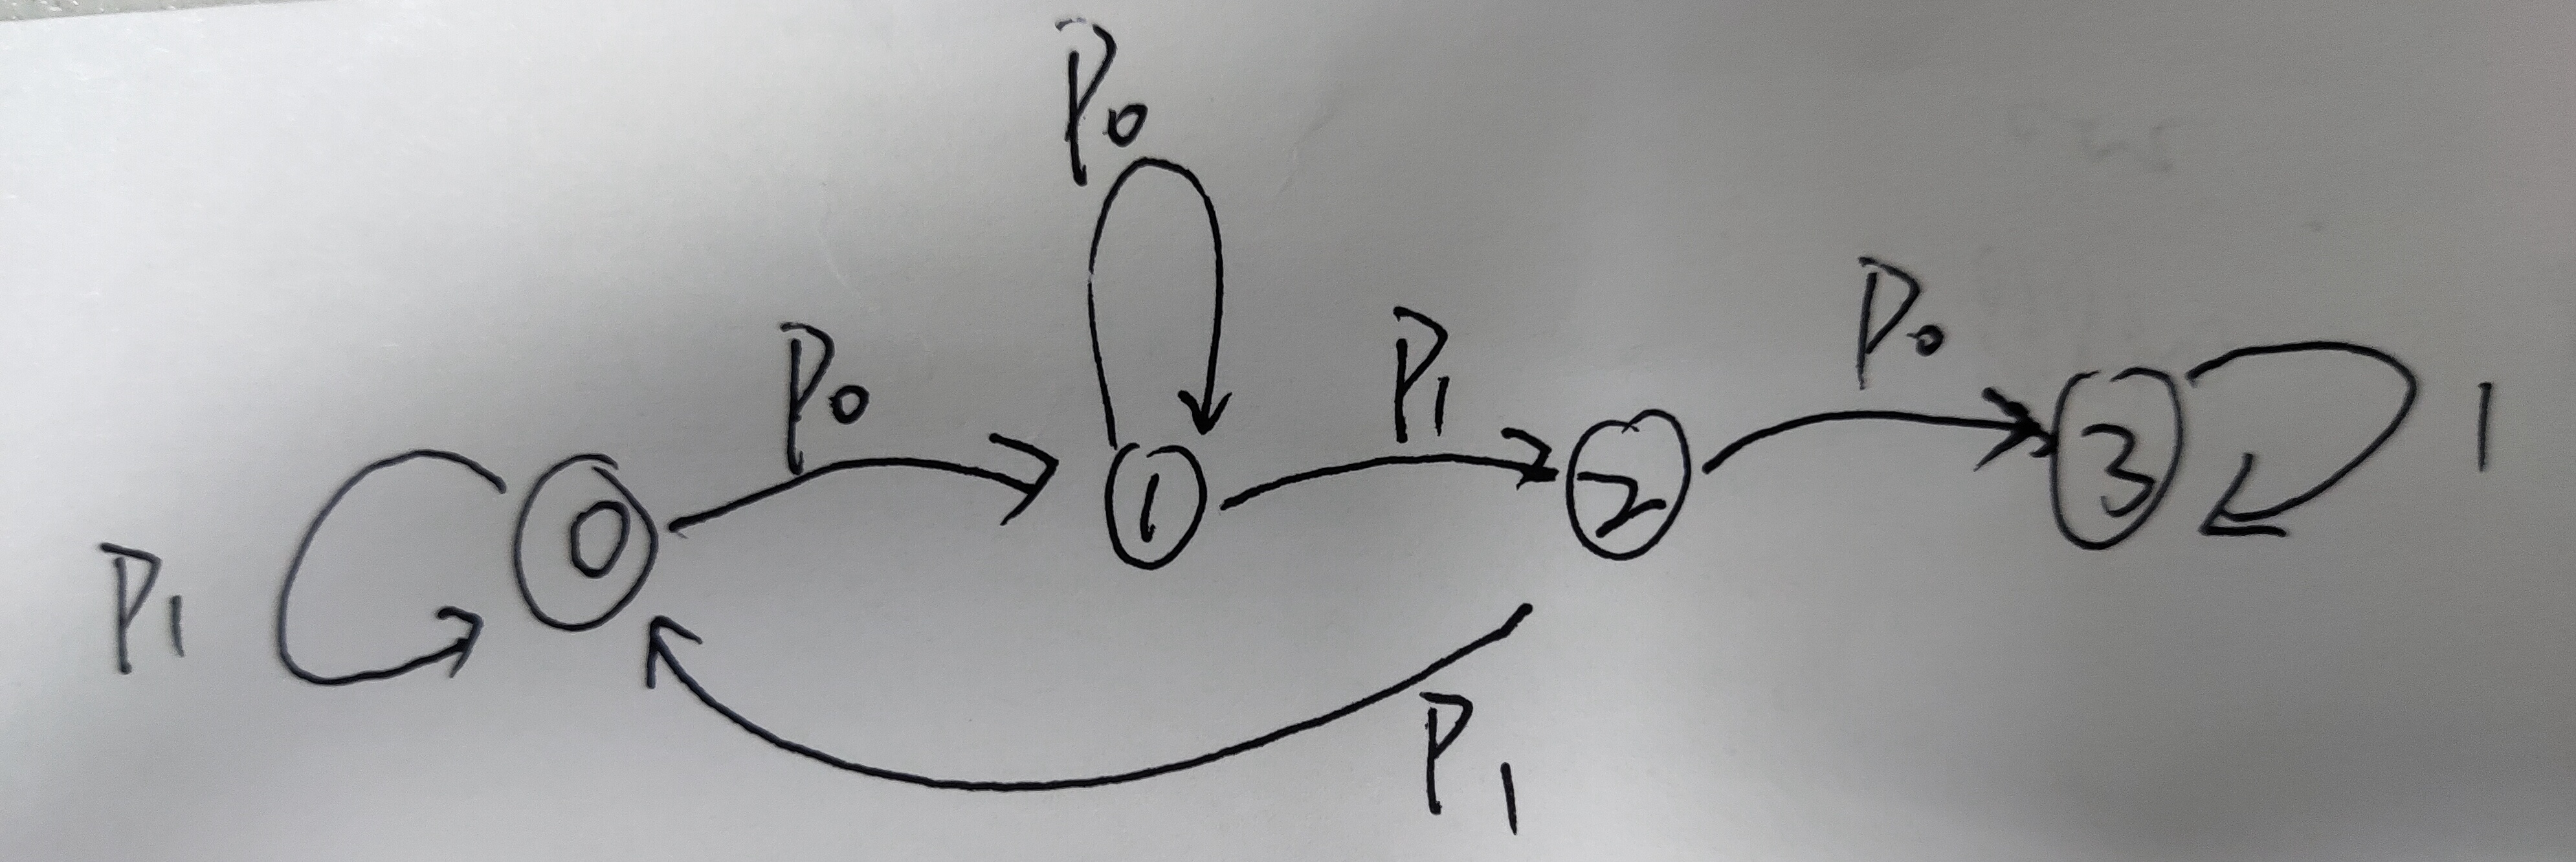
\includegraphics[width=4.0in]{4.jpg}
        \end{figure}
        Since,
        \begin{equation*}
            \begin{aligned}
                \nu_0 &= 1+ p_1\nu_0+p_0\nu_1\\
                \nu_1 &= 1+ p_0\nu_1+p_1\nu_2\\
                \nu_2 &= 1+ p_0\nu_3+p_1\nu_0\\
                \nu_3 &= 0
            \end{aligned}
        \end{equation*}
        Then,
        \begin{equation*}
            \nu_0=\frac{1}{p_0}+\frac{1}{p_1p_0^2}
        \end{equation*}        
    \end{enumerate}
\end{document}